%!TEX root = ../slides.tex

% \section[Introduction]{Introduction \& Context}

% \subsection[Introduction]{Introduction}

\begin{frame}{Context}
  \vfill
  \begin{figure}[htp]
  \centering
  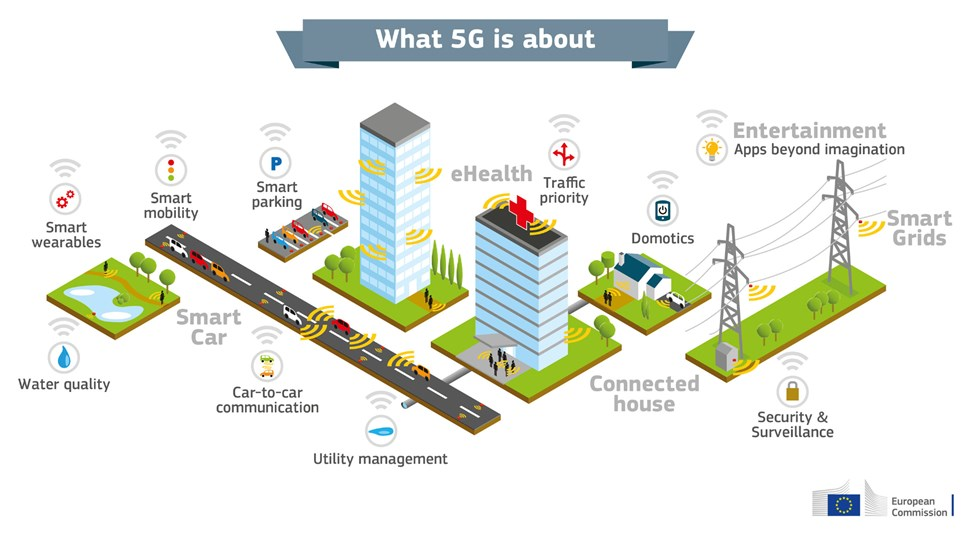
\includegraphics[scale=0.45]{pics/5G}
  \end{figure}
  \vfill
  % \begin{itemize}
  %   \item Nowadays digital communication systems are everywhere
  %   \item Real-time systems are traditionally implemented in hardware
  %   \item Needs validation of more robust and more complex systems
  %   \item Needs to flexibility to adapt to many parameters
  %   \item New challenge: implement digital communication systems in software
  %     \\\vspace*{.5em}
  %     {\color{bleuUni}\Large\MVRightarrow} \textbf{Require high performance implementations}
  % \end{itemize}
\end{frame}

% \subsection[Applicative Contexts]{Applicative Contexts}

\begin{frame}{Software-defined Radio}
  % A Software-Defined Radio (SDR) is a radio communication system where
  % components traditionally implemented in hardware are instead implemented by
  % means of software.
  \vspace{0.3cm}
  \textbf{Software-Defined Radio (SDR)} = radio communication system all in software

  \vfill
  \pause
  \textbf{Evolution of the mobile phone networks:}

  \begin{columns}[T] % align columns
  \begin{column}{.3\textwidth}
    \only<2->{
    \begin{figure}[!h]
    \centering
    \begin{tikzpicture}[scale=0.5, every node/.style={transform shape}]
      \newcommand\yshift{0};

      \PhoneGroup{(-0.5,\yshift)}{0.5};

      \node[draw=black] (rf1) at (2,\yshift) {RF};
      \node[draw=black] (bb1) at (3,\yshift) {BB};

      \draw[black, -] (rf1)--++(0:-0.8cm) node[antenna, scale=0.6] {};
      \draw[-] (rf1) -- (bb1);

      \renewcommand\yshift{-2.0};

      \PhoneGroup{(-0.5,\yshift)}{0.5};

      \node[draw=black] (rf2) at (2,\yshift) {RF};
      \node[draw=black] (bb2) at (3,\yshift) {BB};

      \draw[black, -] (rf2)--++(0:-0.8cm) node[antenna, scale=0.6] {};
      \draw[-] (rf2) -- (bb2);

      \renewcommand\yshift{-4.0};

      \PhoneGroup{(-0.5,\yshift)}{0.5};

      \node[draw=black] (rf3) at (2,\yshift) {RF};
      \node[draw=black] (bb3) at (3,\yshift) {BB};

      \draw[black, -] (rf3)--++(0:-0.8cm) node[antenna, scale=0.6] {};
      \draw[-] (rf3) -- (bb3);

      \draw[black, dashed] (bb1) -- (3.7,0) -- (4.40,-2);
      \draw[black, dashed] (bb2) -- (5.25,-2);
      \draw[black, dashed] (bb3) -- (3.7,-4) -- (4.40,-2);

      \node[draw=Paired-1, dashed, rounded corners =2pt, minimum width=1.0cm, minimum height=0.5cm, label={[Paired-1]above:Base station}, fit=(rf1) (bb1)] {};
    \end{tikzpicture}
    \end{figure}
    }
  \end{column}
  \begin{column}{.3\textwidth}
    \only<3->{
    \begin{figure}[!h]
    \centering
    \begin{tikzpicture}[scale=0.5, every node/.style={transform shape}]
      \newcommand\yshift{0};

      \SmartPhoneGroup{(-0.5,\yshift)}{0.5};

      \node[draw=black] (rf1) at (2,\yshift) {RF};
      \node[draw=black] (bb1) at (5,\yshift-1.45) {BB};

      \draw[black, -] (rf1)--++(0:-0.8cm) node[antenna, scale=0.6] {};
      \draw[-, dashed] (rf1.east) -- (bb1.west);

      \renewcommand\yshift{-2.0};

      \SmartPhoneGroup{(-0.5,\yshift)}{0.5};

      \node[draw=black] (rf2) at (2,\yshift) {RF};
      \node[draw=black] (bb2) at (5,\yshift) {BB};

      \draw[black, -] (rf2)--++(0:-0.8cm) node[antenna, scale=0.6] {};
      \draw[-, dashed] (rf2.east) -- (bb2.west);

      \renewcommand\yshift{-4.0};

      \SmartPhoneGroup{(-0.5,\yshift)}{0.5};

      \node[draw=black] (rf3) at (2,\yshift) {RF};
      \node[draw=black] (bb3) at (5,\yshift+1.45) {BB};

      \draw[black, -] (rf3)--++(0:-0.8cm) node[antenna, scale=0.6] {};
      \draw[-, dashed] (rf3.east) -- (bb3.west);

      \draw[<->,>=latex, black, text=black, label={[black]above:40 km}] (2.4,-1.8) -- (4.6,-1.8) node [midway, above] {40 km};

      \node[draw=Paired-3, dashed, rounded corners=2pt, minimum width=0.5cm, minimum height=1.0cm, label={[Paired-3]below:BB station}, fit=(bb1) (bb2) (bb3)] {};
    \end{tikzpicture}
    \end{figure}
    }
  \end{column}
  \begin{column}{.3\textwidth}
    \only<4->{
    \begin{figure}[!h]
    \centering
    \begin{tikzpicture}[scale=0.5, every node/.style={transform shape}]
      \newcommand\yshift{0};

      \SmartPhoneGroup{(-0.5,\yshift)}{0.5};

      \node[draw=black] (rf1) at (2,\yshift) {RF};

      \draw[black, -] (rf1)--++(0:-0.8cm) node[antenna, scale=0.6] {};

      \renewcommand\yshift{-2.0};

      \SmartPhoneGroup{(-0.5,\yshift)}{0.5};

      \node[draw=black] (rf2) at (2,\yshift) {RF};

      \draw[black, -] (rf2)--++(0:-0.8cm) node[antenna, scale=0.6] {};

      \renewcommand\yshift{-4.0};

      \SmartPhoneGroup{(-0.5,\yshift)}{0.5};

      \node[draw=black] (rf3) at (2,\yshift) {RF};

      \draw[black, -] (rf3)--++(0:-0.8cm) node[antenna, scale=0.6] {};

      \draw[-, dashed] (rf1.east) -- (5,-2);
      \draw[-, dashed] (rf2.east) -- (5,-2);
      \draw[-, dashed] (rf3.east) -- (5,-2);

      \Cloud{(5,-2)}{}{0.5};
      \node[text=black] at (4.7,-2) {BB};

      \node[draw=Paired-5, dashed, rounded corners =2pt, minimum width=2.1cm, minimum height=1.7cm, label={[Paired-5]below:Cloud}] at (4.7, -2) {};
    \end{tikzpicture}
    \end{figure}
    }
  \end{column}
  \end{columns}
  \vfill
  \begin{itemize}
    % \item<2-> Base station = Radio Frequency (RF) + Base Band (BB) processing
    % \item<4-> Virtualization of the BB processing = Cloud Radio Access Network (C-RAN)
    \item<4-> BB virtualization = Cloud Radio Access Network (C-RAN)
    % \item<4-> SDR is considered in the Fifth Generation of Mobile Phone Networks (5G)
    \item<4-> SDR considered for 5G
  \end{itemize}
\end{frame}

\begin{frame}{Digital Communication Systems}
  \begin{figure}[!h]
  \centering
  \begin{tikzpicture}[scale=0.65, every node/.style={transform shape}]
    % \path[use as bounding box] (-2.2, -1.2) rectangle (11.8, 5.2);
    \path[use as bounding box] (-2.7, -1.7) rectangle (12.0, 5.3);
    % \draw (-2.2, -1.2) rectangle (11.8, 5.2);

    \only<1>{
    \tikzset{ txt/.style={draw=white, rounded corners=0pt, minimum height=1cm, minimum width=2.5cm, text=white, align=center} }
    \tikzset{ rxt/.style={draw=white, rounded corners=0pt, minimum height=1cm, minimum width=2.5cm, text=white, align=center} }
    }
    \only<2->{
    \tikzset{ txt/.style={draw=Paired-1, rounded corners=0pt, minimum height=1cm, minimum width=2.5cm, text=Paired-1, align=center} }
    \tikzset{ rxt/.style={draw=Paired-3, rounded corners=0pt, minimum height=1cm, minimum width=2.5cm, text=Paired-3, align=center} }
    }
    \tikzset{ rftx/.style={draw=Paired-1, rounded corners=0pt, minimum height=0.7cm, minimum width=1.0cm, text=black, align=center, rounded corners=2pt, dashed, fill=Paired-1!20} }
    \tikzset{ rfrx/.style={draw=Paired-3, rounded corners=0pt, minimum height=0.7cm, minimum width=1.0cm, text=black, align=center, rounded corners=2pt, dashed, fill=Paired-3!20} }

    \node[style={txt}] (sen) at (0,4) {Source\\Encoder};
    \node[style=txt] (enc) at (4,4) {Channel\\Encoder};
    \node[style=txt] (mod) at (8,4) {Digital\\Modulator};

    \node[style=rftx] (rftx) at (10.5,4) {\textbf{RF}};

    \Cloud{(11,2)}{}{0.65};
    \node[text=black] (chn) at (10.7,2) {Channel};

    \node[style=rfrx] (rfrx) at (10.5,0) {\textbf{RF}};

    \node[style=rxt] (dem) at (8,0) {Digital\\Demodulator};

    \node[style=rxt] (dec) at (4,0) {Channel\\Decoder};
    \node[style={rxt}] (sde) at (0,0) {Source\\Decoder};

    \only<1>{
    \node[draw=Paired-1, fill=Paired-1!20, rounded corners=2pt, minimum height=1.5cm, dashed, fit=(sen) (enc) (mod), align=center, label=center: {\large\textbf{Digital transmission chain (BB)}}] (tx) {};
    \node[draw=Paired-3, fill=Paired-3!20, rounded corners=2pt, minimum height=1.5cm, dashed, fit=(dem) (dec) (sde), align=center, label=center: {\large\textbf{Digital reception chain (BB)}}] (rx) {};
    }
    \only<2->{
    \node[draw=Paired-1, rounded corners=2pt, label={[Paired-1]below:Digital transmitter (BB)}, minimum height=1.5cm, dashed, fit=(sen) (enc) (mod)] (tx) {};
    \node[draw=Paired-3, rounded corners=2pt, label={[Paired-3]above:Digital receiver (BB)   }, minimum height=1.5cm, dashed, fit=(dem) (dec) (sde)] (rx) {};
    }

    \draw[<-,>=latex] (tx.west)  -- (-2,  4) node [left,    above           ] {$\bm{m}$};
    \draw[->,>=latex] (tx.east)  -- (rftx)   node [midway,  above           ] {$\bm{x}$};
    \draw[-         ] (rftx)     -- (11.5,4) node [antenna, above, scale=0.5] {};
    \draw[-         ] (rfrx)     -- (11.5,0) node [antenna, above, scale=0.5] {};
    \draw[<-,>=latex] (rx.east)  -- (rfrx)   node [midway,  below           ] {$\bm{y}$};
    \draw[->,>=latex] (rx.west)  -- (-2,  0) node [left,    below           ] {$\bm{\hat{m}}$};
    \only<2->{
    \draw[->,>=latex] (sen)      -- (enc)    node [midway,  above           ] {$\bm{u}$};
    \draw[->,>=latex] (enc)      -- (mod)    node [midway,  above           ] {$\bm{c}$};
    \draw[->,>=latex] (dem)      -- (dec)    node [midway,  below           ] {$\bm{l}$};
    \draw[->,>=latex] (dec)      -- (sde)    node [midway,  below           ] {$\bm{\hat{u}}$};
    \draw[- ,>=latex] (sen.west) -- (-1.5,4);
    \draw[- ,>=latex] (mod.east) -- ( 9.5,4);
    \draw[- ,>=latex] (dem.east) -- ( 9.6,0);
    \draw[- ,>=latex] (sde.west) -- (-1.5,0);
    }
  \end{tikzpicture}
  \end{figure}

  \begin{itemize}
    \item<1-> Channel: disturbances (noise, interferences)
    \item<2-> Source coding: seek for maximum conciseness in the expression of a message
    \item<2-> Channel coding: make a message robust to channel disturbances
  \end{itemize}
\end{frame}

\begin{frame}{Functional Simulation}
  \begin{figure}[!h]
  \centering
  \begin{tikzpicture}[scale=0.65, every node/.style={transform shape}]
    \path[use as bounding box] (-2.7, -1.7) rectangle (12.0, 5.3);
    % \draw (-2.7, -1.7) rectangle (12.0, 5.3);

    \tikzset{ rftx/.style={draw=Paired-1, rounded corners=0pt, minimum height=0.7cm, minimum width=1.0cm, text=black, align=center, rounded corners=2pt, dashed, fill=Paired-1!20} }
    \tikzset{ rfrx/.style={draw=Paired-3, rounded corners=0pt, minimum height=0.7cm, minimum width=1.0cm, text=black, align=center, rounded corners=2pt, dashed, fill=Paired-3!20} }

    \only<1-3>{
    \tikzset{ txt/.style={draw=Paired-1, rounded corners=0pt, minimum height=1cm, minimum width=2.5cm, text=Paired-1, align=center} }
    \tikzset{ rxt/.style={draw=Paired-3, rounded corners=0pt, minimum height=1cm, minimum width=2.5cm, text=Paired-3, align=center} }
    }
    \only<4->{
    \tikzset{ txt/.style={draw=black, rounded corners=0pt, minimum height=1cm, minimum width=2.5cm, text=black, align=center} }
    \tikzset{ rxt/.style={draw=black, rounded corners=0pt, minimum height=1cm, minimum width=2.5cm, text=black, align=center} }
    }

    \only<1-4>{
    \tikzset{ chn/.style={draw=black, rounded corners=0pt, minimum height=1cm, minimum width=2.0cm, text=black, align=center} }
    \tikzset{ cde/.style ={} }
    }
    \only<5->{
    \tikzset{ chn/.style ={draw=Paired-1, rounded corners=0pt, minimum height=1cm, minimum width=2.0cm, text=Paired-1, align=center} }
    \tikzset{ cde/.style ={draw=Paired-3, text=Paired-3} }
    }

    \only<1>{
    \tikzset{ hid2/.style={} }
    }
    \only<2->{
    \tikzset{ hid2/.style ={draw=white, text=white, align=center} }
    }
    \only<1>{
    \node[style={txt,hid2}] (sen) at (0,4) {Source\\Encoder};
    }
    \only<3->{
    \node[style={txt}] (src) at (0,4) {Source};
    }
    \node[style={txt,cde}] (enc) at (4,4) {Channel\\Encoder};
    \only<1>{
    \node[style=txt] (mod) at (8,4) {Digital\\Modulator};
    }
    \only<2->{
    \node[style=txt] (mod) at (8,4) {BPSK\\Modulator};
    }
    \only<1-2>{
    \node[style=rftx] (rftx) at (10.5,4) {\textbf{RF}};
    }
    \only<1-2>{
    \Cloud{(11,2)}{}{0.65};
    }
    \only<1>{
    \node[text=black] (chn) at (10.7,2) {Channel};
    }
    \only<2>{
    \node[text=black, align=center] (chn) at (10.7, 2) {AWGN\\Channel};
    }
    \only<3->{
    \node[style={chn}   ] (chn) at (10.7, 2) {AWGN\\Channel};
    }
    \only<1-2>{
    \node[style=rfrx] (rfrx) at (10.5,0) {\textbf{RF}};
    }
    \only<1>{
    \node[style=rxt] (dem) at (8,0) {Digital\\Demodulator};
    }
    \only<2->{
    \node[style=rxt] (dem) at (8,0) {BPSK\\Demodulator};
    }
    \node[style={rxt,cde}] (dec) at (4,0) {Channel\\Decoder};
    \only<1>{
    \node[style={rxt,hid2}] (sde) at (0,0) {Source\\Decoder};
    }
    \only<3->{
    \node[style={rxt}] (mnt) at (0,0) {Monitor};
    }

    \only<1>{
    \node[draw=Paired-1, rounded corners=2pt, label={[Paired-1]below:Digital transmitter (BB)}, minimum height=1.5cm, dashed, fit=(sen) (enc) (mod)] (tx) {};
    \node[draw=Paired-3, rounded corners=2pt, label={[Paired-3]above:Digital receiver (BB)   }, minimum height=1.5cm, dashed, fit=(dem) (dec) (sde)] (rx) {};
    }
    \only<2>{
    \node[draw=Paired-1, rounded corners=2pt, label={[Paired-1]below:Digital transmitter (BB)}, minimum height=1.5cm, dashed, fit=(enc) (mod)] (tx) {};
    \node[draw=Paired-3, rounded corners=2pt, label={[Paired-3]above:Digital receiver (BB)   }, minimum height=1.5cm, dashed, fit=(dem) (dec)] (rx) {};
    }
    \only<3>{
    \node[draw=Paired-1, rounded corners=2pt, label={[Paired-1]below:Digital transmitter (BB)}, minimum height=1.5cm, dashed, fit=(src) (enc) (mod)] (tx) {};
    \node[draw=Paired-3, rounded corners=2pt, label={[Paired-3]above:Digital receiver (BB)   }, minimum height=1.5cm, dashed, fit=(mnt) (dem) (dec)] (rx) {};
    }
    \only<4->{
    \node[draw=Paired-5, rounded corners=2pt, label={[Paired-5]below:Simulation chain}, minimum height=4.15cm, dashed, fit=(src) (enc) (mod) (chn) (dem) (dec) (mnt)] (sim) {};
    }

    \only<1>{
    \draw[<-,>=latex, style=hid2] (tx.west)  -- (-2,  4) node [left,    above           ] {$\bm{m}$};
    }
    \only<1-2>{
    \draw[->,>=latex] (tx.east)  -- (rftx)   node [midway,  above           ] {$\bm{x}$};
    \draw[-         ] (rftx)     -- (11.5,4) node [antenna, above, scale=0.5] {};
    \draw[-         ] (rfrx)     -- (11.5,0) node [antenna, above, scale=0.5] {};
    \draw[<-,>=latex] (rx.east)  -- (rfrx)   node [midway,  below           ] {$\bm{y}$};
    \draw[- ,>=latex, style=hid2] (sen.west) -- (-1.5,4);
    \draw[- ,>=latex] (mod.east) -- ( 9.5,4);
    \draw[- ,>=latex] (dem.east) -- ( 9.6,0);
    \draw[- ,>=latex, style=hid2] (sde.west) -- (-1.5,0);
    }

    \only<3>{
    \draw[->,>=latex] (mod) -| (chn)                   node [midway, above] {$\bm{x}$};
    \draw[->,>=latex] (chn) |- (dem)                   node [midway, below] {$\bm{y}$};
    \draw[->,>=latex] (2,4) -- (2,0.35) -- (1.25,0.35) node [midway, below] {};
    }
    \only<4->{
    \draw[->,>=latex] (mod) -| (chn)                   node [midway, above] {};
    \draw[->,>=latex] (chn) |- (dem)                   node [midway, below] {};
    \draw[->,>=latex] (2,4) -- (2,0.35) -- (1.25,0.35) node [midway, below] {};
    }

    \only<1>{
    \draw[->,>=latex, style=hid2] (rx.west)  -- (-2,  0) node [left,    below           ] {$\bm{\hat{m}}$};
    }
    \only<1-2>{
    \draw[->,>=latex            ] (sen)      -- (enc)    node [midway,  above           ] {$\bm{u}$};
    }
    \only<3>{
    \draw[->,>=latex            ] (src)      -- (enc)    node [midway,  above           ] {$\bm{u}$};
    }
    \only<4>{
    \draw[->,>=latex            ] (src)      -- (enc)    node [midway,  above           ] {};
    }
    \only<1-3>{
    \draw[->,>=latex            ] (enc)      -- (mod)    node [midway,  above           ] {$\bm{c}$};
    }
    \only<4>{
    \draw[->,>=latex            ] (enc)      -- (mod)    node [midway,  above           ] {};
    }
    \only<1-3>{
    \draw[->,>=latex            ] (dem)      -- (dec)    node [midway,  below           ] {$\bm{l}$};
    }
    \only<4>{
    \draw[->,>=latex            ] (dem)      -- (dec)    node [midway,  below           ] {};
    }
    \only<1-2>{
    \draw[->,>=latex            ] (dec)      -- (sde)    node [midway,  below           ] {$\bm{\hat{u}}$};
    }
    \only<3>{
    \draw[->,>=latex            ] (dec)      -- (mnt)    node [midway,  below           ] {$\bm{\hat{u}}$};
    }
    \only<4>{
    \draw[->,>=latex            ] (dec)      -- (mnt)    node [midway,  below           ] {};
    }

    \only<5->{
    \draw[->,>=latex, text=Paired-3] (src) -- (enc) node [midway, above] {$K$};
    \draw[->,>=latex, text=Paired-3] (enc) -- (mod) node [midway, above] {$N$};
    \draw[->,>=latex, text=Paired-3] (dem) -- (dec) node [midway, below] {$N$};
    \draw[->,>=latex, text=Paired-3] (dec) -- (mnt) node [midway, below] {$K$};

    \node[text width=0.3cm, text centered, text=Paired-3] (C) at (-2.5, 3.875) {$C$};
    \node[text width=0.3cm, text centered, text=Paired-3] (K) at (-2.5, 3.125) {$K$};
    \node[text width=0.3cm, text centered, text=Paired-3] (N) at (-2.5, 2.375) {$N$};


    \draw[->,>=latex, dashed, Paired-3] (C) -- (sim);
    \draw[->,>=latex, dashed, Paired-3] (K) -- (sim);
    \draw[->,>=latex, dashed, Paired-3] (N) -- (sim);

    \node[text width=4cm, text centered, text=Paired-3] (C2) at (4, 2) {$C$ = \{Polar, LDPC, Turbo, ...\}};

    \draw[->, dotted, Paired-3, line width=0.7pt] (C2) -- (enc);
    \draw[->, dotted, Paired-3, line width=0.7pt] (C2) -- (dec);
    }
    \only<6->{
    \node[text width=0.3cm, text centered, text=Paired-1] (m) at (-2.5, 1.625) {$m$};
    \node[text width=0.3cm, text centered, text=Paired-1] (M) at (-2.5, 0.875) {$M$};
    \node[text width=0.3cm, text centered, text=Paired-1] (s) at (-2.5, 0.125) {$s$};

    \draw[->,>=latex, dashed, Paired-1] (m) -- (sim);
    \draw[->,>=latex, dashed, Paired-1] (M) -- (sim);
    \draw[->,>=latex, dashed, Paired-1] (s) -- (sim);
    }

    \only<6->{
    \draw[<-,>=latex, Paired-1] (10.1,2.3) to[bend right=20] (8.5,2.2) node [left, yshift=0.4cm, xshift=-0.2cm] {};
    \node[text=Paired-1, align=center] at (7.5, 2) {input: $E_b/N_0$};
    }

    \only<7>{
    \draw[->,>=latex, Paired-5] (0,0.2) to[bend left=30] (0,1.8) {};
    \node[text=Paired-5, align=center] at (0.3,2) {output: BER/FER};
    }
  \end{tikzpicture}
  \end{figure}

  \only<2>{
  \begin{itemize}
    \item BPSK: binary phase-shift keying modulation
    \item AWGN: additive white Gaussian noise
      \\\vspace*{.5em}
      {\color{bleuUni}\Large\MVRightarrow} Commonly used to evaluate error correcting codes
  \end{itemize}
  }
  \only<3-4>{
  \begin{itemize}
    \item<3-> Source: generates random frames
    \item<3-> Monitor: compares the initial message $\bm{u}$ with the decoded message $\bm{\hat{u}}$
    \item<4-> All the processing represent a \textbf{simulation chain}
  \end{itemize}
  }
  \only<5->{
  \begin{itemize}
    \item<5-> \textcolor{Paired-3}{$C$}, \textcolor{Paired-3}{$K$} and \textcolor{Paired-3}{$N$} are the characteristics of the channel code
    \item<6-> \textcolor{Paired-1}{$m$}, \textcolor{Paired-1}{$M$} and \textcolor{Paired-1}{$s$} are the configurations of the channel model
    \item<7-> Decoding performance are estimated by the monitor with \textcolor{Paired-5}{Bit Error Rate (BER)} and \textcolor{Paired-5}{Frame Error Rate (FER)} metrics
  \end{itemize}
  }
\end{frame}

% \subsection[Problematics]{Problematics and Contributions}

\begin{frame}{Challenges}
  \vfill

  \begin{enumerate}
    \item Propose \textbf{fast software implementations} of digital processing algorithms
    % \begin{item}
    %   \item
    % \end{item}
    \vspace{0.3cm}
    \item Combine \textbf{efficiency, flexibility and portability} in the implementations
    \vspace{0.3cm}
    \item Manage \textbf{algorithmic heterogeneity} and \textbf{reproduce state-of-the-art} results
    \vspace{0.3cm}
    \item Enable efficient execution of full \textbf{SDR chains on parallel architectures}
  \end{enumerate}

  % \underline{Software-defined Radio:}
  % \vspace*{.5em}
  % \begin{itemize}
  %   \item<1-> \textbf{High throughput}: required for high resolution video streaming
  %   \item<2-> \textbf{Low latency}: required for remote medical operations
  %   \item<3-> \textbf{Flexibility}: the ability to adapt to many configurations
  %   \item<4-> \textbf{Portability}: take advantage of the large variety of General Purpose Processors (GPPs) and operating systems
  % \end{itemize}
  % \vfill
  % \pause
  % \pause
  % \pause
  % \pause
  % \underline{Functional Simulation:}
  % \vspace*{.5em}
  % \begin{itemize}
  %   \item<5-> \textbf{Simulation time}: expensive Monte Carlo simulation of the whole chain
  %   \item<6-> \textbf{Algorithmic heterogeneity}: many algorithms with various characteristics
  %   \item<7-> \textbf{Reproducibility}: ease the reproduction of the state-of-the-art results
  % \end{itemize}
  \vfill
\end{frame}

\begin{frame}{Contributions}
  \begin{enumerate}
    \item<1-> Flexible high performance implementations of channel decoders (Polar codes, Turbo codes and LDPC codes)~\cite{Cassagne2015c,Cassagne2016a,Cassagne2016b,Leonardon2019,Ghaffari2019}
    \begin{itemize}
      \item High throughput and low latency on single core and multi-core CPUs
      \item Flexibility
    \end{itemize}
    \vspace{.3em}
    \item<2-> Portable and efficient low level description of the signal processing algorithms~\cite{Cassagne2018}
    \begin{itemize}
      \item High throughput and low latency on single-core CPUs
      \item Flexibility \& Portability
    \end{itemize}
    \vspace{.3em}
    \item<3-> Open-source library and functional simulator dedicated to the digital communication systems~\cite{Cassagne2017,Cassagne2017a,Cassagne2019a}
    \begin{itemize}
      \item Simulation time
      \item Algorithmic heterogeneity
      \item Reproducibility
    \end{itemize}
    \vspace{.3em}
    \item<4-> Embedded domain specific language (eDSL) for the SDR
    \begin{itemize}
      \item High throughput and low latency on multi-core CPUs
    \end{itemize}
  \end{enumerate}
\end{frame}
